\chapter{\xlabel{scuba2_overview}SCUBA-2 Overview}
\label{sec:s2}
\section{\xlabel{scuba2}The instrument}


The Submillimetre Common User Bolometer Array-2 (SCUBA-2) is a
10,000-pixel bolometer camera. It has two arrays operating
simultaneously to map the sky in the atmospheric windows of 450 and
850$\mu$m. Each array is made up of four sub-arrays as shown in
\cref{Figure}{fig:arrays}{}.

\subsubsection*{How it works}
The SCUBA-2 bolometers are integrated arrays of superconducting
transition edge sensors (TESs) with a characteristic transition
temperature, $T_c$. In addition, each TES is ringed with a resistive
heater which can compensate for changes in sky power. The SCUBA-2
focal plane is kept at a base temperature slightly below $T_c$,
however a voltage is applied across each TES resistance to position
the bolometer at the transition temperature. From this point, any
increase of temperature on the bolometers (e.g. from an astronomical
signal) will increase the TES resistance and heat it up. This causes a
drop in current and therefore a drop in temperature making the system
self-regulating.

For properly performing bolometers, the change in current through the
TES is proportional to the change in resistance, with the response
calibrated using flat-field observations (described below). This
changing current generates a magnetic field which is amplified by a
chain of superconducting quantum interference devices (SQUIDs). This
induces a feedback current which is proportional to the current
flowing through the TES, and it is this feedback current that is
recorded during data acquisition.


\subsubsection*{Setups}

Before science data can be taken the system must be optimised. These
`setups' are performed after slewing to the azimuth of the source,
where the SQUID, TES and heater biases are set to pre-determined
nominal values, in order to position the bolometers in the middle of
the transition range.

\subsubsection*{Flat-field}

 The shutter then opens onto the sky, and
as it does so the gradual increase in sky power hitting the array is
compensated for by a decrease in the resistive heater power via a
servo loop designed to keep the TES output constant. This acts to keep
the bolometers positioned at the centre of the transition range and is
known as \textbf{heater tracking}.

The responsivity of the bolometers will change slightly between the
dark and the sky; therefore, once the shutter is fully open a fast
\textbf{flat-field} observation is carried out to recalibrate them.
\textbf{A flat-field measures the responsivity of each bolometer to
changing sky power}. It does this by utilising the resistance heaters
which are ramped up and down around the nominal value. The change in
current through the TES is then recorded for each bolometer giving a
measure of its responsivity. The flat field solution is then the
inverse linear gradient of the current as a function of heater power.

At this point bolometers with responsivities above or below a
threshold limit are rejected, along with bolometers that display a
non-linear response or have a poor S/N. A second flat-field is
performed at the end of an observation so bolometers whose
responsivity has changed over the course of the observation can be
flagged.

For full details of the array setup and operation see Holland et al.
(2013) \cite{s2main}.

\begin{figure}[t!]
\begin{center}
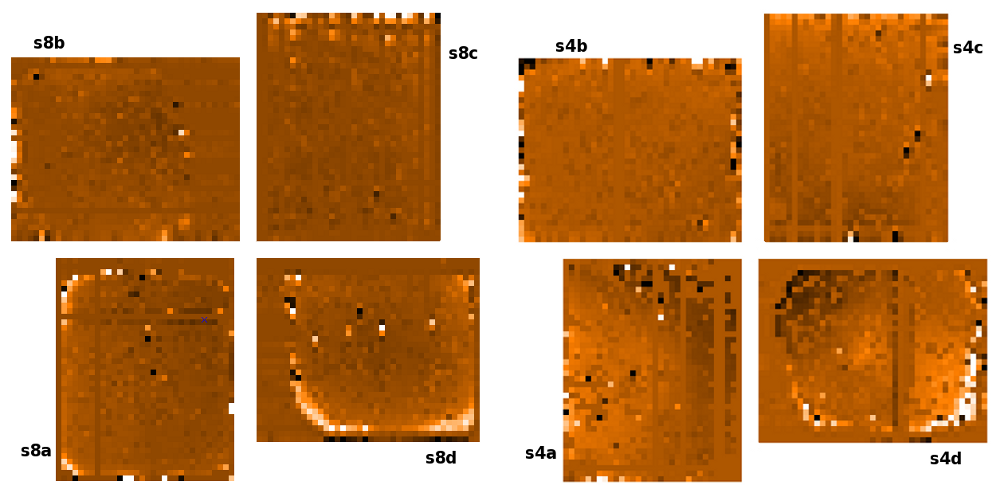
\includegraphics[width=0.8\linewidth]{sc21_arrays}
\label{fig:arrays}
\caption[The physical layout of the arrays at each wavelength]{
  \small The layout of the arrays at 850$\mu$m (left) and
  450$\mu$m (right). The labels denote the name assigned to each
  sub-array. Raw data files are generated separately for each sub-array
  and must be co-added. This figure was made by running
 \wcsmosaic\ on a raw sub-scan from each sub-array.
}
\end{center}
\end{figure}

\section{\xlabel{obs_modes}Observing modes}
\label{sec:mmodes}

Two observing modes are offered for SCUBA-2: \textsc{daisy} and
\textsc{pong}. As the bulk of \mbox{SCUBA-2} observing involves
large area mapping, both observing modes are scan patterns. Your
choice depends on the size of the area you wish to map, where you
would like your integration time concentrated and the degree of
extended emission you wish to recover.


\begin{aligndesc}

\item[\textbf{PONG}] A \textsc{pong} map is the scan strategy for
  covering a large area. The default options allow for three
  sizes---900\,arcsec, 1800\,arcsec and 3600\,arcsec. A single
  \textsc{pong} map is a square of these dimensions and the telescope
  fills in the square by bouncing off the edge of the area. To ensure
  an even sky background it is recommended a minimum of three, but
  preferably more than five, \textsc{pong} maps are included in a
  single observation with a rotation introduced between each one. In
  this way a circular pattern is built up, (see the lower right-hand
  panel of \cref{Figure}{fig:scan}{graphic below}), with a diameter
  equal to your requested map size.

  To recover large-scale extended structure you are advised to use
  larger \textsc{pong} maps which scan at a higher rate. This option
  is preferable to tiling multiple smaller maps. Ultimately it is the
  size of the SCUBA-2 field-of-view that determines the sensitivity to
  large-scale structure.

\item[\textbf{DAISY}] \textsc{daisy} maps are the option for
  point-like or compact sources ($<$3~arcmin) by maximising the
  exposure time on the centre of the image. The telescope moves at a
  constant velocity in a `spirograph' pattern that has the advantage
  of keeping the source on the array throughout the observation. This
  is shown in the top panel of \cref{Figure}{fig:scan}{the figure
    below}. While the central $<$3~arcmin has a uniform background noise,
    \textsc{daisy} maps cover a circular area of diameter of 12~arcmin.

\end{aligndesc}

\textbf{Should I use a \textsc{daisy} or a 15-arcmin \textsc{pong}?}  A
common issue is that a pong900 is used when possibly
a \textsc{daisy} would have been better, given that the latter is much faster and employs a significant
exposure time out to a diameter of 12~arcmin. The numbers break down as follows:

\begin{figure}
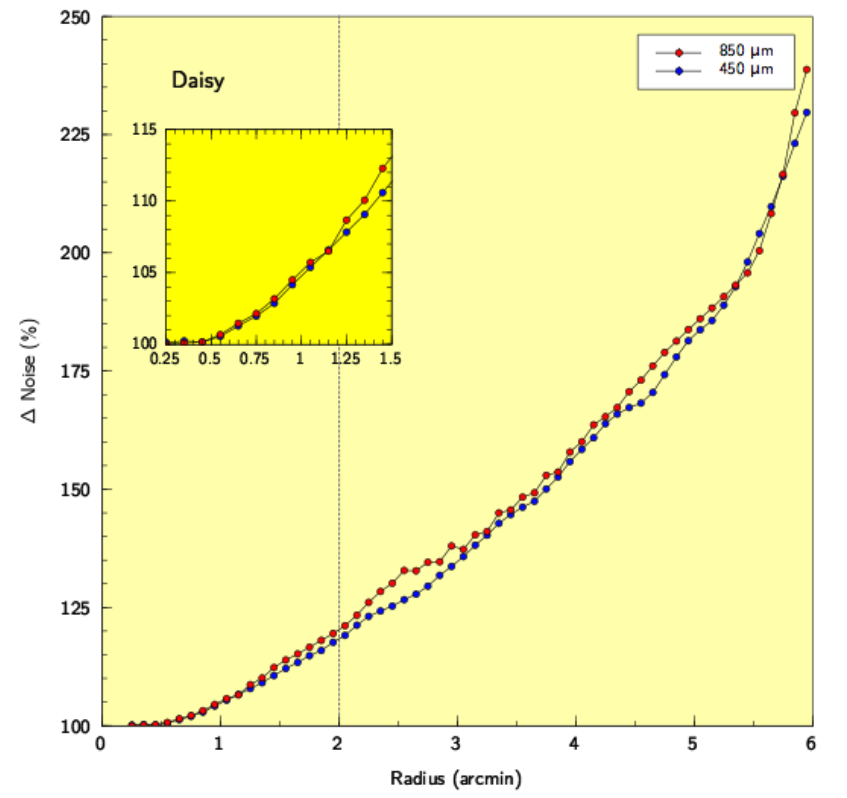
\includegraphics[width=0.47\linewidth]{sc21_DaisyRadProf.png}
\hspace{3mm}
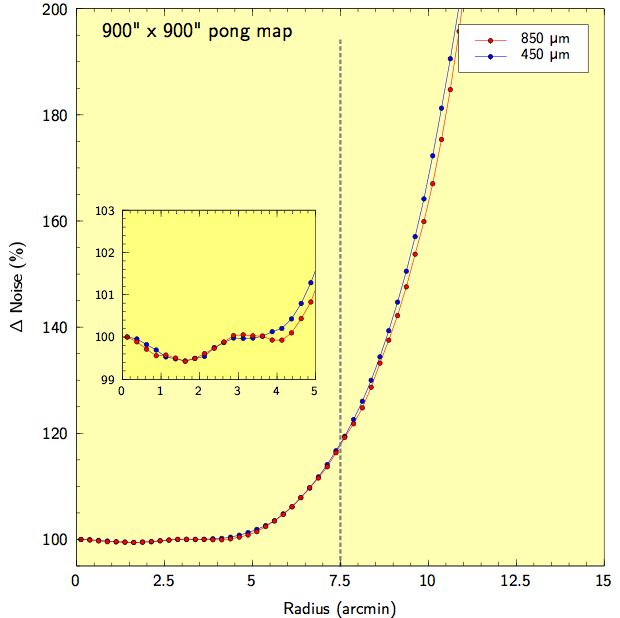
\includegraphics[width=0.445\linewidth]{sc21_Pong900RadProf.png}
\caption[Radial noise profiles for \textsc{Daisy} and \textsc{pong} maps.]{The
radial noise profiles for a \textsc{daisy} and \textsc{pong900} map. For the same integration time, the rms in the center ($<$3~arcmin) of a \textsc{daisy} will be more than twice as good as in a \textsc{pong900}. Out to a radius of $\sim$5.5~arcmin, the noise will still be below the \textsc{pong900} target noise.}
\label{fig:PongDaisyRadProf}
\end{figure}

\vspace{5mm}

\textit{For the same integration time}, the rms in the center ($<$3~arcmin) of a Daisy will be more than twice as good as in a pong900. Out to a radius of $\sim$5.5~arcmin, the noise will still be below the pong900 target noise. Beyond this radius the noise will exceed the target noise, but that is also the case for the pong900 (see the radial profiles in
\cref{Figure}{fig:PongDaisyRadProf}{}).

\vspace{5mm}

I.e. the trade-off is between a flatter and slightly larger map (pong900) and a somewhat smaller but much deeper map in the center with a distinct noise gradient across the field (\textsc{daisy}).

\vspace{5mm}

Detection experiments may well be better off with Daisies, although statistical conclusions, such as number counts, may become more complicated. The same may be true for isolated (i.e. non-mosaicked) fields where one could ask if the negative impact of the noise gradient and a smaller field out-weigh the benefits of a deeper mapping across most of the image.

There are other possibilities, such as doing an initial exploratory \textsc{daisy} to the required depth in a 3~arcmin field (this can be done in less that 25\% of the time it takes for a \textsc{pong900}) and then proceed with pongs on the most promising candidate(s). \textsc{pong} and \textsc{daisy} fields can be combined. It may also be beneficial to use a pattern of offset \textsc{daisies} to mitigate somewhat for the more pronounced gradient or to better match the source morphology in the field.

\subsubsection*{Why these patterns?}

SCUBA-2 removes atmospheric noise in the data-processing
stage (Holland et al. 2013) \cite{s2main}. The power spectrum
of data taken by SCUBA-2 has a $1/f$ noise curve at lower frequencies. To
ensure astronomical signals are far away from this $1/f$ noise, fast
scanning speeds are required.

In order to disentangle persistent source structure from other
slowly varying signals (e.g. extinction, sky noise, $1/f$ noise), the
scan pattern must pass across each region of the map from different
directions (hour angles) and at different times. The scan patterns themselves, along
with the associated parameters (velocity and scan-spacing), have been
designed and optimised to meet both these criteria. \textsc{daisies},
\textsc{pong900}, \textsc{pong1800}, and \textsc{pong3600} have telescope
velocities of 155$^{\prime\prime}$/s, 280$^{\prime\prime}$/s, 400$^{\prime\prime}$/s,
and 600$^{\prime\prime}$/s, respectively.

\starfig{sc21_wayne_scan}{[t!]}{width=0.98\linewidth}{fig:scan}{%
  Illustration of the SCUBA-2 observing patterns}{%

  The top row shows a \textsc{daisy} and the bottom row shows a
  \textsc{pong}.  The left column shows the telescope track over a
  single rotation of the pattern.  The right column shows the telescope
  track after multiple rotations of the pattern.  The scan pattern for
  an observation can be visualised in this way with \topcat\ using the
  output from \jcmtstate.  See \cref{section}{sec:scan}{Displaying
  scan patterns} for more details.  Figure modified from Holland et al. (2013).
}


\section{The raw data}
\label{sec:rawdata}
A normal science observation will follow the following sequence.

\begin{enumerate}\itemsep-0.2em
\item Flat-field
\item Science scans
\item Flat-field
\end{enumerate}

The \param{SEQ\_TYPE} keyword in the FITS header may be used to
identify the nature of each scan (see
\cref{Section}{sec:fitsheader}{Headers and file structure}).  When you
access raw from the \htmladdnormallink{Science
  Archive}{http://www3.cadc-ccda.hia-iha.nrc-cnrc.gc.ca/jcmt/} you
will get all of the files listed above. Later when you reduce your
data using the map-maker you must include all the science files
\emph{and} the first flat-field.  The final flat-field is not
currently used.

Shown below is a list of the raw files for a single sub-array (in this
case s8a) for a short calibration observation. The first and last
scans are the flat-field observations,which occur after the shutter
opens to the sky at the start of the observation and closes at the end
(note the identical file size); all of the scans in between are
science.


\begin{terminalv}
% ls -lh /jcmtdata/raw/scuba2/s8a/20131227/00034
\end{terminalv}

\begin{terminalv}
-rw-r--r-- 1 jcmtarch jcmt 8.0M Dec 27 03:00 s8a20131227_00034_0001.sdf
-rw-r--r-- 1 jcmtarch jcmt  22M Dec 27 03:00 s8a20131227_00034_0002.sdf
-rw-r--r-- 1 jcmtarch jcmt  22M Dec 27 03:01 s8a20131227_00034_0003.sdf
-rw-r--r-- 1 jcmtarch jcmt  22M Dec 27 03:02 s8a20131227_00034_0004.sdf
-rw-r--r-- 1 jcmtarch jcmt  22M Dec 27 03:02 s8a20131227_00034_0005.sdf
-rw-r--r-- 1 jcmtarch jcmt 6.8M Dec 27 03:02 s8a20131227_00034_0006.sdf
-rw-r--r-- 1 jcmtarch jcmt 8.0M Dec 27 03:03 s8a20131227_00034_0007.sdf
\end{terminalv}

The SCUBA-2 data-acquisition (DA) system writes out a data file every
30 seconds; each of which contains 22\,MB of data. The only exception
is the final science scan which will usually be smaller (6.8\,MB in
the example above), typically requiring less than 30 seconds of data
to complete the observation.

\textbf{Note:} All of these files are written out eight times, once
for each of the eight sub-arrays.

The main data arrays of each file are cubes, with the first two
dimensions enumerating bolometer columns and rows within a sub-array,
and the third time slices (sampled at roughly 200\,Hz).

A standardised file naming scheme is used in which each file name starts
with the sub-array name, followed by the UT date of the observation in
the format \texttt{yyyymmdd}, followed by a five-digit observation
number, followed by the sub-scan number. The name ends with the standard
suffix \texttt{.sdf} used by all Starlink data files. For instance, the files
listed above hold data from the s8a sub-array for observation 34 taken on
27th December 2013.

\subsubsection*{Units}

Raw SCUBA-2 data come in uncalibrated units. The first calibration
step is to scale the raw data to units of picowatts (pW)
by applying the flat-field solution. This step is performed internally
by the map-maker but can be done manually when examining the raw
data---see \cref{Section}{sec:concat}{Concatenate \& apply a
  flat-field}.

The second step is to scale the resulting map by the flux conversion factor
(FCF) to give units of janskys. When running the
\textsc{Orac-dr} pipeline this is done automatically.
% STM: We are now encouraging users to stick with the nominal FCF values since there can be a significant
% variation over short timescales throughout the night. The long-term trends are, therefore, more robust, rather
% than picking one or two calibrator observations on a given night that may be affected by a variety of factors.
% Keeping this in mind, I am commenting out the lines below:
%However it is good to check that the FCF value applied to your data is sensible.
%Checking FCF's must be done manually, instructions for this is
%given in \cref{Section}{sec:own_fcf}{Determining your own flux-conversion
%  factors}.


